\chapter{\IfLanguageName{dutch}{Short List}{Short List}}%
\label{ch:shortlist}

In dit hoofdstuk wordt kort besproken hoe de shortlist van vijf databases is samengesteld. Voorafgaand aan het selecteren van de verschillende databases is een lijst met de rankings van de meest populaire databases wereldwijd geraadpleegd. Deze lijst, opgesteld door~\autocite{DBEngines}, omvat meer dan 300 databases. Hoewel deze lijst een uitgebreid overzicht biedt, is het belangrijk op te merken dat niet alle vermelde databases relevant zijn voor het opstellen van een e-commerce webshop in de mode-industrie. Het doorzoeken en vergelijken van elke database op deze lijst is echter een onbegonnen werk. 


Het bedrijf van de co-promotor van deze literatuurstudie (Aware) maakt momenteel gebruik van MariaDB (gerangschikt op de 13\textsuperscript{\text{de}} plaats, \ref{fig:mariadbranking}) en Amazon Aurora (gerangschikt op de 50\textsuperscript{ste} plaats, \ref{fig:amazonauroraranking}) voor hun operationele behoeften. Om deze reden werden deze twee databases als eerste opgenomen in de vergelijking.

\begin{figure}[H]
    \centering
    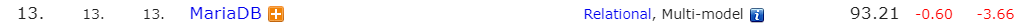
\includegraphics[width=\linewidth]{graphics/mariadbranking}
    \caption[MariaDB ranking]{MariaDB ranking~\autocite{DBEngines}}
    \label{fig:mariadbranking}
\end{figure}

\begin{figure}[H]
    \centering
    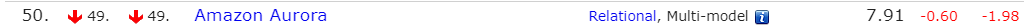
\includegraphics[width=\linewidth]{graphics/amazonauroraranking}
    \caption[Amazon Aurora ranking]{Amazon Aurora ranking~\autocite{DBEngines}}
    \label{fig:amazonauroraranking}
\end{figure}

Na zorgvuldige overweging en analyse werden nog drie andere databases geselecteerd om de shortlist van vijf databases aan te vullen. Deze databases zijn Couchbase, ClickHouse en MongoDB.
\begin{figure}[H]
    \centering
    \includegraphics[width=\linewidth]{"graphics/mongodb ranking"}
    \caption[MongoDB ranking]{MongoDB ranking~\autocite{DBEngines}}
    \label{fig:mongodb-ranking}
\end{figure}
\begin{figure}[H]
    \centering
    \includegraphics[width=\linewidth]{"graphics/couchbase ranking"}
    \caption[Couchbase ranking]{Couchbase ranking~\autocite{DBEngines}}
    \label{fig:couchbase-ranking}
\end{figure}
\begin{figure}[H]
    \centering
    \includegraphics[width=\linewidth]{"graphics/clickhouse ranking"}
    \caption[ClickHouse ranking]{ClickHouse ranking~\autocite{DBEngines}}
    \label{fig:clickhouse-ranking}
\end{figure}


Couchbase werd gekozen voor de key-features die aangeboden worden, speciaal voor retail en e-commerce. Deze key-features omvatten: ~\autocite{Couchbasea} 

\begin{itemize}
    \item Makkelijkere en betaalbaardere schaalbaarheid.
    \item Verbeterde prestaties dankzij een in-memory en gedistribueerde architectuur die sub-millisecond reactietijden levert.
    \item De hoge beschikbaarheid.
    \item Kostenbesparingen en versnelling van de time-to-market door flexibiliteit en operationele efficiëntie, waardoor bedrijven snel kunnen reageren op veranderende marktomstandigheden.
\end{itemize}

Met MariaDB en Amazon Aurora, twee relationele databases en de NoSQL database, Couchbase, ontbrak er nog een tweede NoSQL database. Hiervoor werd geopteerd voor MongoDB. MongoDB staat wereldwijd bekend als een van de meest prominente NoSQL-databases en staat ook gerangschikt op de vijfde plaats.

Als laatste database werd gekozen voor een kolom database, ClickHouse. ClickHouse werd gekozen vanwege zijn uitstekende prestaties, schaalbaarheid, betrouwbaarheid, flexibele architectuur, uitgebreide functionaliteiten en gebruiksvriendelijkheid. Het biedt razendsnelle verwerking van analytische queries, schaalt efficiënt mee met hardwarebronnen tot petabyte-schaal, ondersteunt betrouwbare replicatie over meerdere datacenters, en vereenvoudigt het schrijven van queries met een gebruiksvriendelijke SQL-dialect.~\autocite{ClickHousea}


